\documentclass{article}

\title{Homework 1 : Graphs and Network Flows}
\author{Aashith Kamath Manjeshwar, Saikrishna Badrinarayanan}
\newcommand{\R}{\mathbf{R}}
\newcommand{\U}{\mathbf{U}}
\newcommand{\V}{\mathbf{V}}
\newcommand{\W}{\mathbf{W}}

\usepackage{graphicx}
\graphicspath{ {plots/} }
\begin{document}
\maketitle

In this project, we use the igraph library to generate different kinds of networks and measure several properties of 
each of these networks. We use the netrw package to run random walks on the graphs
generated. The project was coded in the language R.

\paragraph{Problem 1}: \\
a)\\
The first problem involved creating an undirected random network with 1000 nodes and a probability $p=0.01$ that
every pair of nodes has an edge between them. \\

b)\\
In this question, we perform random walks on the graph generated above. 
A random walk (with no damping) is a process in which you start at one node and at each step,
move to one of it's neighbours such that each neighbour has the same probability of being moved to.
We start from each vertex and 
perform random walks using 10 walkers and for 50 timesteps. We set the term called damping as 1 to denote that
there is no damping in the random walk.
We measure the average distance that the 
walker has walked as a function of the steps. That is, suppose we use $t$ to denote the number of steps.
For each $t$ from 1 to 50, we measure the average distance $s(t)$ that a walker has walked in all the random
walks we have performed above. Similarly, we also measure the variance and standard deviation of the 
distance for each timestep. Finally, we plot three graph with timesteps on the x-axis and average distance, variance
and standard deviation respectively on the y-axis.\\
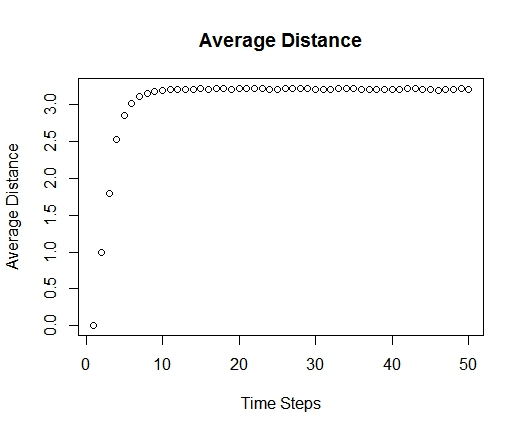
\includegraphics[scale=0.4]{p1a} \\
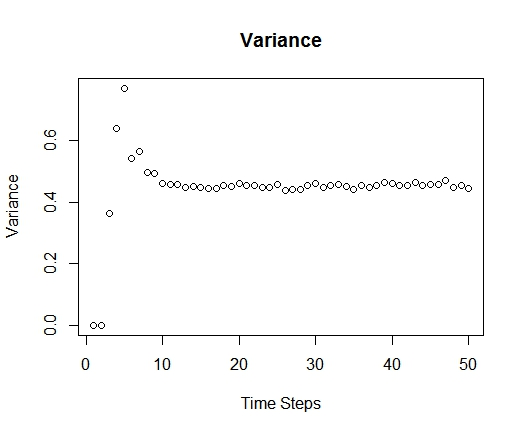
\includegraphics[scale=0.4]{p1b} \\
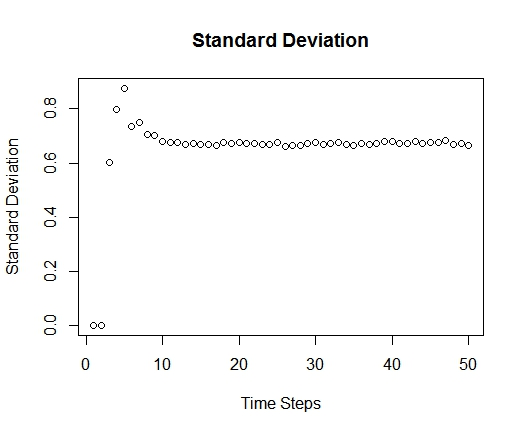
\includegraphics[scale=0.4]{p1c} \\
We also measure the diameter of the graph which turns out to be 5.\\

c)\\
We know that in a d-dimensional space, a random walker has average signed distance to be 0.
On the other hand, in a graph, the average distance that a walker travels after any number of timesteps is 
always positive. As a result of this, the average distance we plotted above does not really conform to the
average signed distance in a d-dimensional space.\\

In the case of standard deviation, the average in a d-dimensional space is proportional to $\sqrt t$
where $t$ is the number of timesteps after which we measure the standard deviation. In the case of our graph,
we notice that the variance stabilises to roughly $0.7$ after certain timesteps and is not proportional to $\sqrt t$.\\

d)\\
In this problem, we repeat (b) but with two new graphs that have 10000 and 100 nodes respectively.\\
i) 10000 nodes graph :\\
The diameter of the graph is 3.\\
The average distance vs timestep plot is :\\
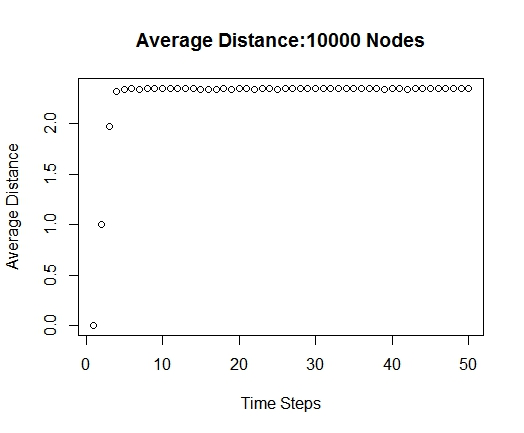
\includegraphics[scale=0.4]{p1i} \\
The standard deviation vs timestep plot is :\\
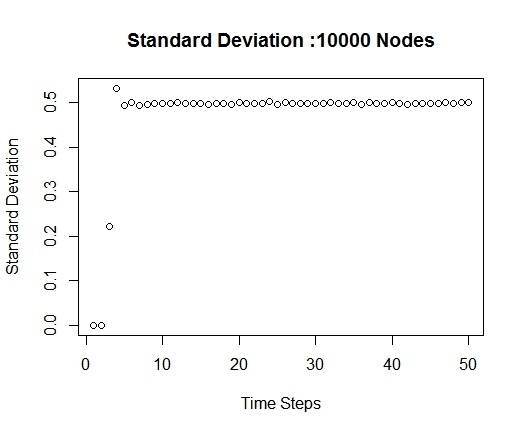
\includegraphics[scale=0.4]{p1k} \\
The variance vs timestep plot is :\\
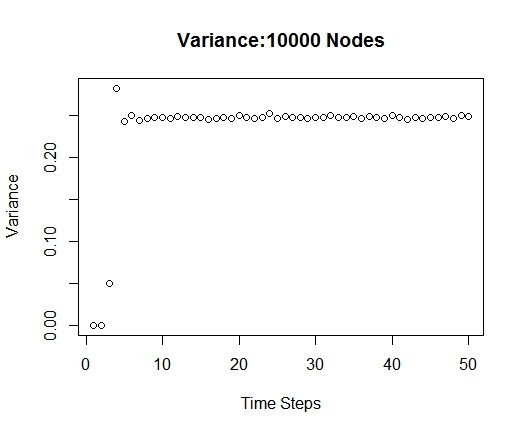
\includegraphics[scale=0.4]{p1j} \\
ii) 100 nodes graph :\\
In the case of 100 nodes, we observe that the graph we generated is not connected.
As a result, when we perform a random walk, we tend to stay within one component only. If we
start at a node that has no neighbour, the walk randomly jumps to a node that is not connected to it
(even though there is no damping) leading to incorrect results. To avoid this issue, we first find the 
giant connected component (GCC) of the graph and then perform the random walks on the GCC.\\
The diameter of the graph is 8.\\
The average distance vs timestep plot is :\\
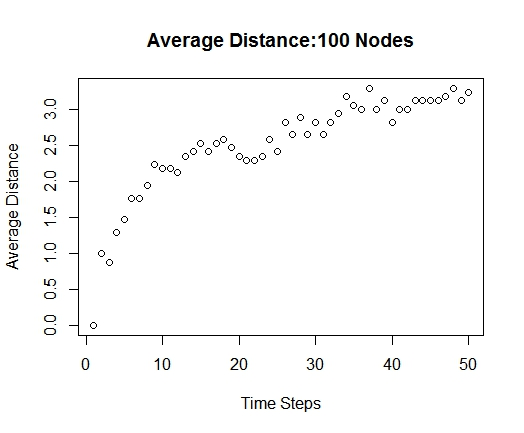
\includegraphics[scale=0.4]{p1d} \\
The standard deviation vs timestep plot is :\\
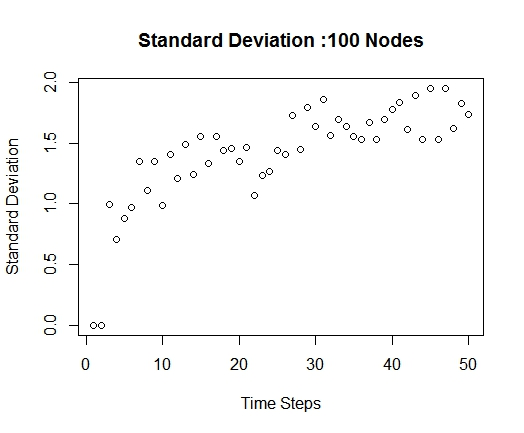
\includegraphics[scale=0.4]{p1f} \\
The variance vs timestep plot is :\\
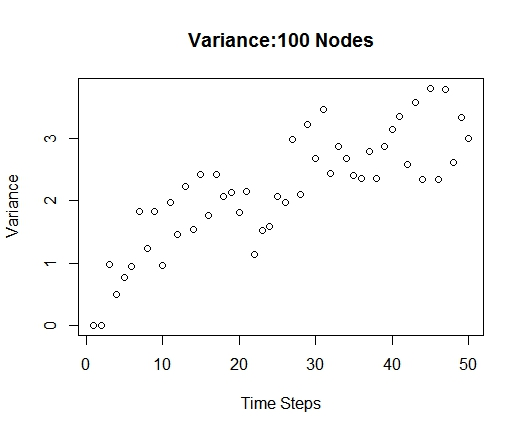
\includegraphics[scale=0.4]{p1e} \\

We observe that as the number of the nodes in the graph increases, the diamater of the graph decreases.
We also observe that, as the number of nodes increases, the average distance and variance take lesser timesteps to 
converge to one value in the random walks. We even see that for the 100 node graph, the values don't seem to
converge even after 50 steps. Thus, as the diameter of the graph decreases, which means that they are 
more ``dense'' or closely knit, the timesteps taken to converge goes down. This is the relationship between the two
quantities.

e)\\
We first plot the degree distribution of the graph.
The degree distribution is a plot containing the various degrees of the nodes in the graph on the x-axis
and their corresponding density (frequency of that degree occuring divided by the total number of nodes) on the y-axis.
After this, we plot the degree distribution of the nodes reached at the end of the random walk 
in the graph containing 1000 nodes. The two plots are :\\
Original graph's degree distribution :\\
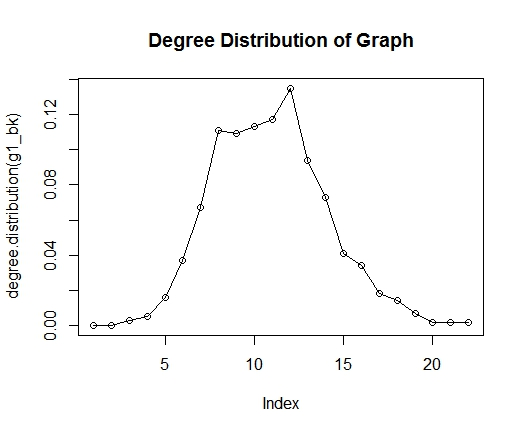
\includegraphics[scale=0.4]{p1g} \\
Degree distribution of nodes reached at the end of the random walk :\\
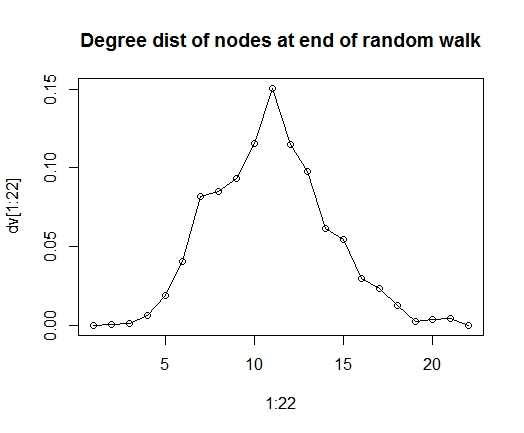
\includegraphics[scale=0.4]{p1h} \\
We observe that the two plots are very similar. That is, the degree distribution of the 
original graph is very similar to the degree distribution of the nodes reached at the end of the 
random walk. This is somewhat expected because a random walk is expected to cover all the nodes in the graph.\\

\hrule

\paragraph{2)}
a)\\
This problem involves creating an undirected random network with 1000 nodes whose degree 
distribution is proportional to $x^{-3}$ (a fat-tailed degree distribution). We use barabasi.game to generate 
such a graph.\\

b)\\
In this question, we perform random walks on the graph generated above. We start from each vertex and 
perform random walks using 10 walkers and for 50 timesteps.  We set the term called damping as 1 to denote that
there is no damping in the random walk. We measure the average distance that the 
walker has walked as a function of the steps. That is, suppose we use $t$ to denote the number of steps.
For each $t$ from 1 to 50, we measure the average distance $s(t)$ that a walker has walked in all the random
walks we have performed above. Similarly, we also measure the variance and standard deviation of the 
distance for each timestep. Finally, we plot three graph with timesteps on the x-axis and average distance, variance
and standard deviation respectively on the y-axis.\\
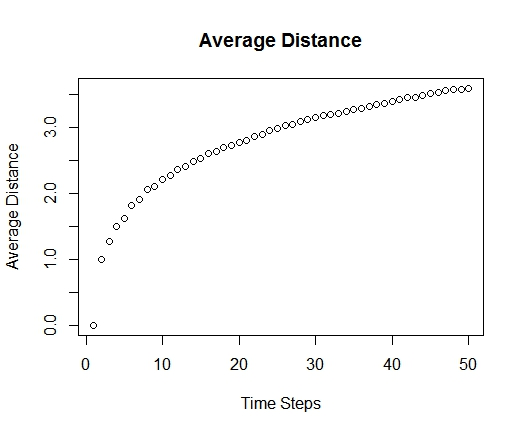
\includegraphics[scale=0.4]{p2a} \\
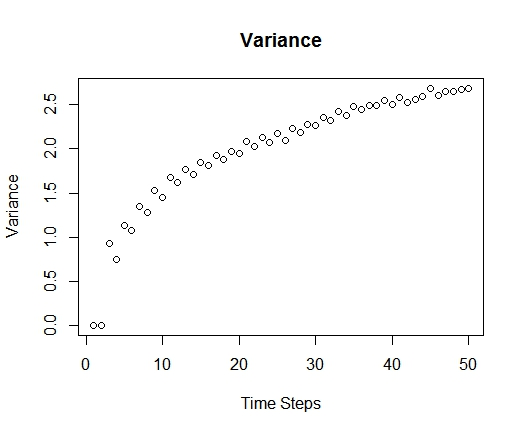
\includegraphics[scale=0.4]{p2b} \\
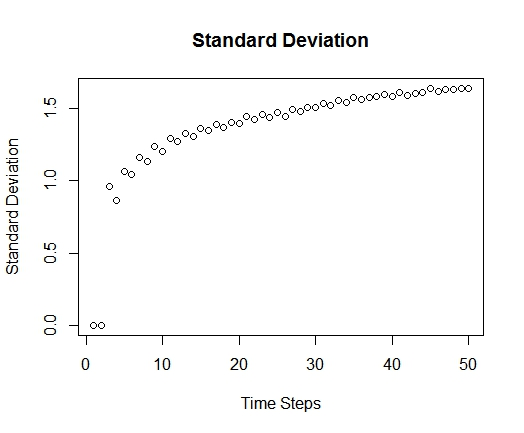
\includegraphics[scale=0.4]{p2c} \\
We also measure the diameter of the graph which turns out to be 18.\\
c)\\
We know that in a d-dimensional space, a random walker has average signed distance to be 0.
On the other hand, in a graph, the average distance that a walker travels after any number of timesteps is 
always positive. As a result of this, the average distance we plotted above does not really conform to the
average signed distance in a d-dimensional space.\\

In the case of standard deviation, the average in a d-dimensional space is proportional to $\sqrt t$
where $t$ is the number of timesteps after which we measure the standard deviation. In the case of our graph,
we notice that the variance stabilises to roughly $0.7$ after certain timesteps and is not proportional to $\sqrt t$.\\

d)\\
In this problem, we repeat (b) but with two new graphs that have 10000 and 100 nodes respectively.\\
i) 10000 nodes graph :\\
The diameter of the graph is 27.\\
The average distance vs timestep plot is :\\
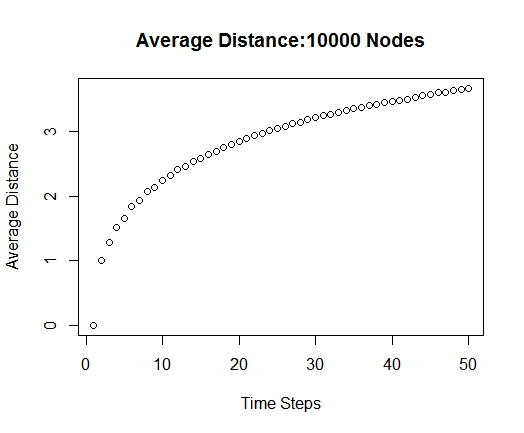
\includegraphics[scale=0.4]{p2i} \\
The standard deviation vs timestep plot is :\\
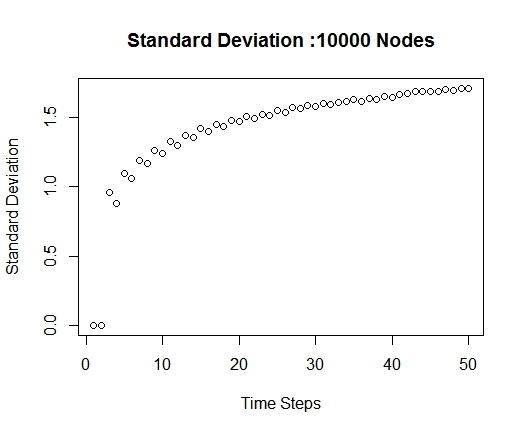
\includegraphics[scale=0.4]{p2k} \\
The variance vs timestep plot is :\\
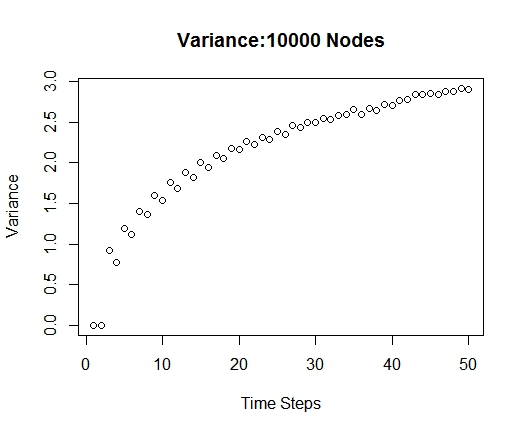
\includegraphics[scale=0.4]{p2j} \\
ii) 100 nodes graph :\\
In the case of 100 nodes, we observe that the graph we generated is not connected.
As a result, when we perform a random walk, we tend to stay within one component only. If we
start at a node that has no neighbour, the walk randomly jumps to a node that is not connected to it
(even though there is no damping) leading to incorrect results. To avoid this issue, we first find the 
giant connected component (GCC) of the graph and then perform the random walks on the GCC.\\
The diameter of the graph is 11.\\
The average distance vs timestep plot is :\\
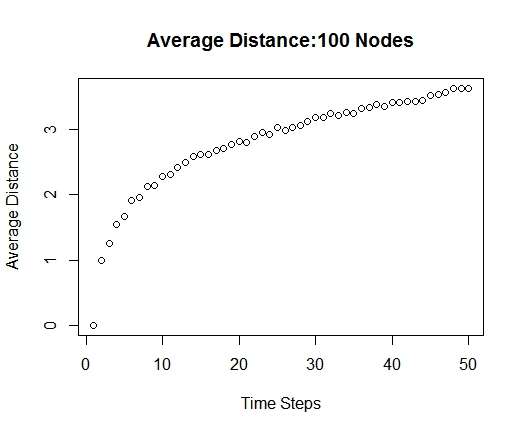
\includegraphics[scale=0.4]{p2d} \\
The standard deviation vs timestep plot is :\\
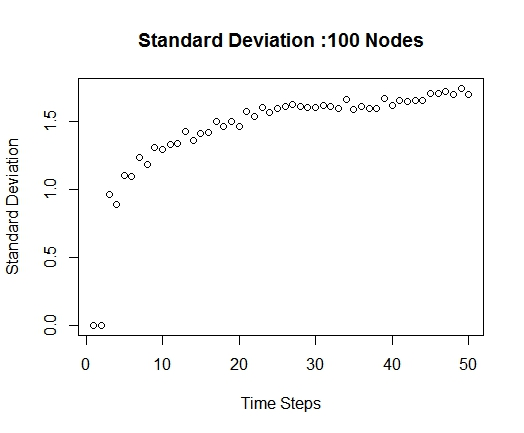
\includegraphics[scale=0.4]{p2f} \\
The variance vs timestep plot is :\\
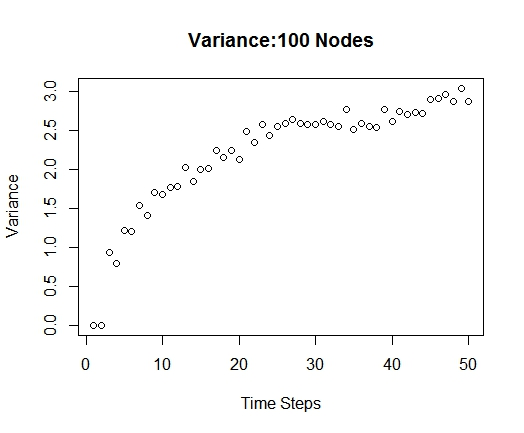
\includegraphics[scale=0.4]{p2e} \\
We observe that as the number of the nodes in the graph increases, the diamater of the graph also increases.
We also observe that, as the number of nodes increases, the average distance and variance take more timesteps to 
converge to one value in the random walks. Thus, as the diameter of the graph decreases, which means that they are 
more ``dense'' or closely knit, the timesteps taken to converge goes down. This is the relationship between the two
quantities.

e)\\
We first plot the degree distribution of the graph.
After this, we plot the degree distribution of the nodes reached at the end of the random walk 
in the graph containing 1000 nodes. The two plots are :\\
Original graph's degree distribution :\\
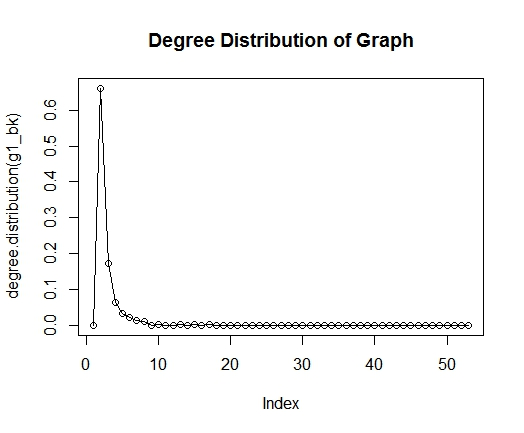
\includegraphics[scale=0.4]{p2g} \\
Degree distribution of nodes reached at the end of the random walk :\\
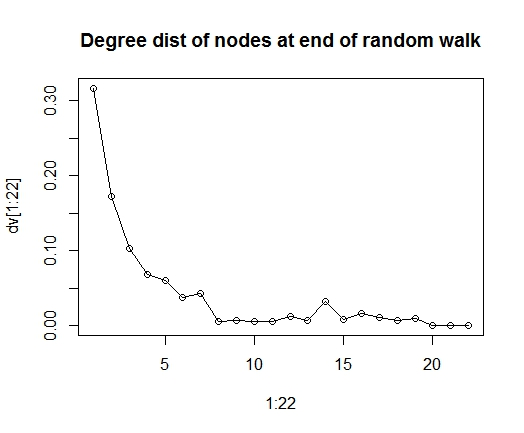
\includegraphics[scale=0.4]{p2h} \\
We observe that the two plots are very similar. That is, the degree distribution of the 
original graph is very similar to the degree distribution of the nodes reached at the end of the 
random walk and they are both fat-tailed degree distributions. This is somewhat 
expected because a random walk is expected to cover all the nodes in the graph.\\

\hrule

\paragraph{3)}
a)\\
For the 1000 node undirected random graph we generated in problem 1, and the corresponding random walks that we performed,
we measure the probability that the walker visits each node by using the ``average visit probability'' term
in the output of the netrw package. Since we have several walkers, we average out this value over all the walkers.
We plot a graph with the x-axis containing the nodes of the graph and the y-axis containing the 
average visit probability of that node.\\
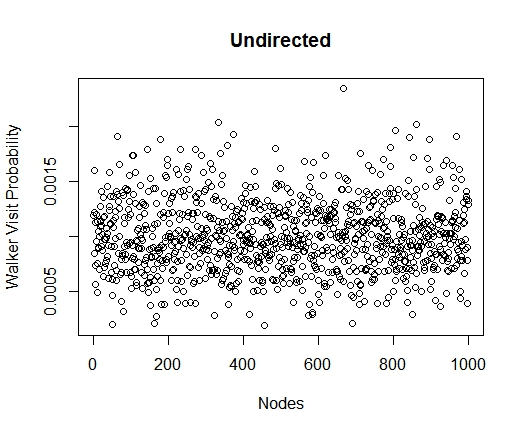
\includegraphics[scale=0.4]{p3a} \\
Next, we try to find a relation between this probability and the degree of the nodes.
We do this by plotting a graph that contains the degree of the nodes on the x-axis and on the y-axis,
for each degree $d$, the corresponding value is the average probability that the walker visits those nodes which
have degree $d$.\\
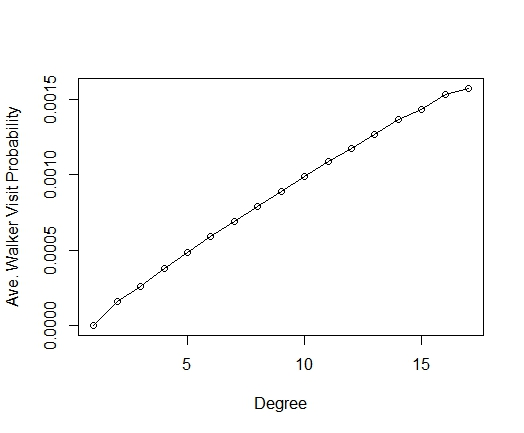
\includegraphics[scale=0.4]{p3b} \\
We notice from the plot that it is almost linear, which means that the probability is directly proportional to the 
degree of the nodes.\\

b)\\
The first part of the problem involved creating a directed random network 
with 1000 nodes and a probability $p=0.01$ that every pair of nodes has an edge between them. \\
For this graph, we perform random walks as done previously in question 1(b).
We measure the probability that the walker visits each node by using the ``average visit probability'' term
in the output of the netrw package. Since we have several walkers, we average out this value over all the walkers.
We plot a graph with the x-axis containing the nodes of the graph and the y-axis containing the 
average visit probability of that node.\\
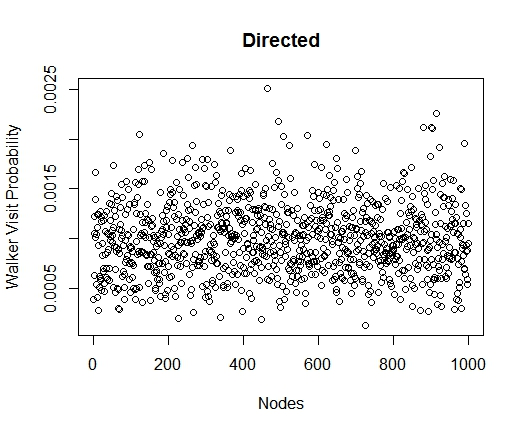
\includegraphics[scale=0.4]{p3c} \\
Next, we try to find a relation between this probability and the degree of the nodes.
We do this by plotting a graph that contains the degree of the nodes on the x-axis and on the y-axis,
for each degree $d$, the corresponding value is the average probability that the walker visits those nodes which
have degree $d$. The problem here is that, unlike in the case of undirected graphs, each node
has an in-degree and an out-degree. We first plot by considering the degree of the node to be the sum of its in and out 
degrees.\\

\textbf{Probability vs Total Degree}\\
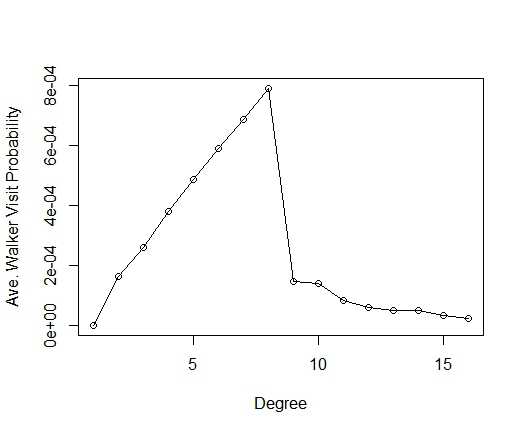
\includegraphics[scale=0.4]{p3d} \\
From the plot,we notice that the line is zig-zagged indicating that the probability
first rises with the degree then it falls. This is contrary to what we got in the case of undirected graphs and is
also not very logical. To remove this strange relation, we repeat the same plot by only considering the in-degree.
This makes more sense because the probability that a node is visited should purely depend on the number of edges
it has coming in to it, as that is what influences the walker to reach that node. The plot is shown below:\\

\textbf{Probability vs in-Degree}\\
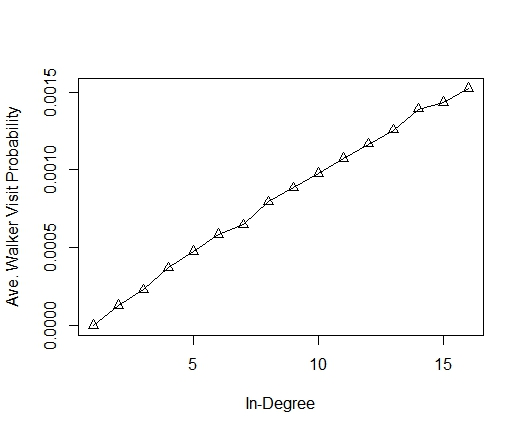
\includegraphics[scale=0.4]{p3e} \\
We notice from the plot that it is almost linear, which means that the probability is directly proportional to the 
degree of the nodes. This is similar to the case of the undirected graph.\\

a)\\
For the 1000 node undirected random graph we generated in problem 1, we perform random walks similar to 1(b) but 
with a small change. We set the damping parameter to be $0.85$. This means that at each node, the walker
moves to one of it's neighbours with probability $0.85$ and teleports to a random node in the graph
with probability $0.15$. Then, we measure the probability that the walker visits each node by using the ``average visit probability'' term
in the output of the netrw package. Since we have several walkers, we average out this value over all the walkers.
We plot a graph with the x-axis containing the nodes of the graph and the y-axis containing the 
average visit probability of that node.\\
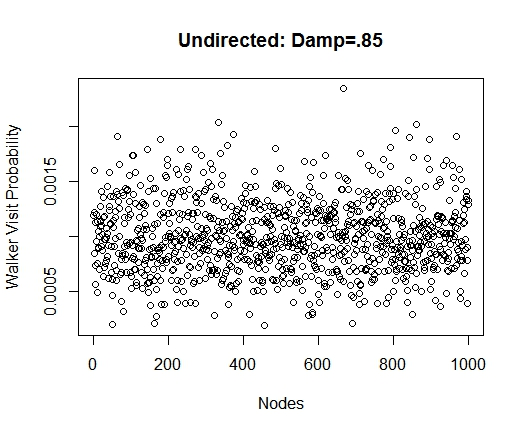
\includegraphics[scale=0.4]{p3f} \\
Next, we try to find a relation between this probability and the degree of the nodes.
We do this by plotting a graph that contains the degree of the nodes on the x-axis and on the y-axis,
for each degree $d$, the corresponding value is the average probability that the walker visits those nodes which
have degree $d$.\\
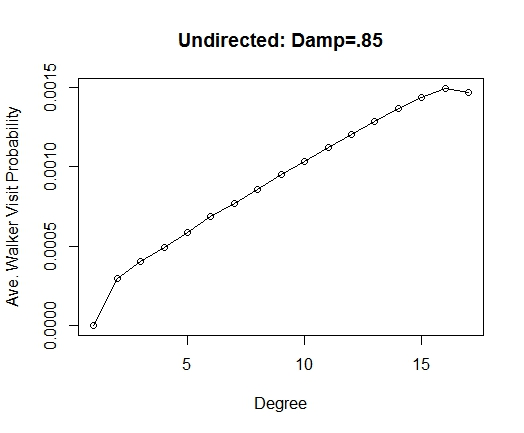
\includegraphics[scale=0.4]{p3g} \\
We notice from the plot that it is almost linear, which means that the probability is directly proportional to the 
degree of the nodes. It is not as smooth as in 3(a) but this can be explained by the fact that
the walker doesn't always move to the node's neighours. The random ``jumps'' induced by the 
teleportation causes some distortion in the relation between the probability and the degree 
and so the graph is less smoother than before.\\

\hrule

\paragraph{4)}
a)\\
The first part of the problem involved creating a directed random network 
with 1000 nodes and a probability $p=0.01$ that every pair of nodes has an edge between them. \\
For this graph, we perform random walks as done previously in question 3(b) but with a small change.
We set the damping parameter to be $0.85$. This means that at each node, the walker
moves to one of it's neighbours with probability $0.85$ and teleports to a random node in the graph
with probability $0.15$. The random walks performed simulate the normal pagerank.
We measure the probability that the walker visits each node by using the ``average visit probability'' term
in the output of the netrw package. Since we have several walkers, we average out this value over all the walkers.
Since our random walks are simulating normal pagerank, the average visit probability of each node 
corresponds to the pagerank of that node. We plot a graph with the x-axis containing the nodes of the graph and the y-axis containing the 
average visit probability of that node.\\
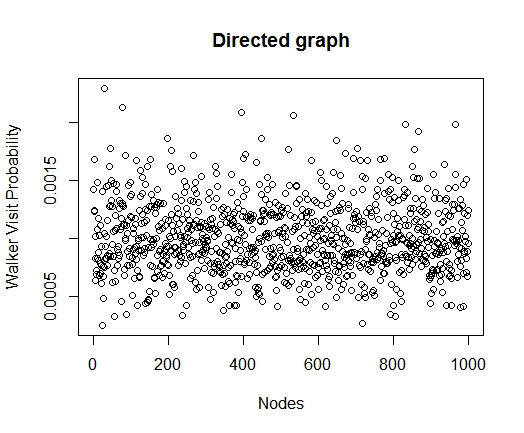
\includegraphics[scale=0.4]{p4a} \\

b)\\
Here, we have our own notion of importance assigned to a node. That is, instead of the normal pagerank, where
the teleportation probability assigned to each node is the same, we use the pagerank values computed in the previous question
and assign them to the teleportation values. That is, we are interpreting this as relying on google's computed pagerank values
to decide which websites to visit and how important they are. We perform random walks and simulate pagerank as in the 
previous question (with damping factor as $0.85$) except for the modification to the teleportation probability as discussed. We call the resulting pagerank
as the personalised pagerank. Then, 
We measure the probability that the walker visits each node by using the ``average visit probability'' term
in the output of the netrw package. Since we have several walkers, we average out this value over all the walkers.
Since our random walks are simulating pagerank, the average visit probability of each node 
corresponds to the personalised pagerank of that node. We plot a graph with the x-axis containing the nodes of the graph and the y-axis containing the 
average visit probability of that node. We have two functions plotted - the red one corresponds to the personalised
pagerank and the black dots stand for the normal pagerank (computed in (a)). We plot them both together
to enable easier comparison between the two.\\
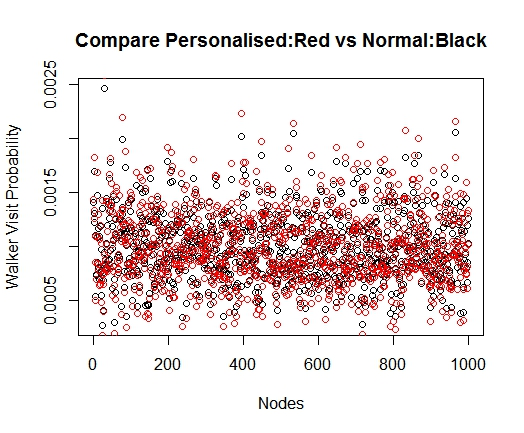
\includegraphics[scale=0.4]{p4b} \\
We observe that whenever the probability is high (above a certain threshold) in the normal case, the probability
is even higher in the case of the personalised pagerank and vice versa. This makes sense because the teleportation probabilities
to the personalised pagerank are fed from the normal one.
Thus, the personalised pagerank might be a better notion.\\

c)\\
Suppose the pages are $P_1,\ldots,P_N$\\
In normal pagerank, the equation is :\\
$$Pr(P_i) = \frac{(1-d)}{N} + \sum\limits_{P_j \in M(P_i)} \frac{Pr(P_j)}{L(P_j)} $$
where $M(P_i)$ is the set of pages that have a link to $P_i$, $Pr(P_i)$ is the pagerank of the page $P_i$
and $d$ is the damping factor (which we set to $0.85$).\\
Here, the teleportation probability to each node is constant and is set to $1/N$. Also, we observe that
the sum of all the pagerank values is equal to 1.\\
Now, in the personalised pagerank (done in (b)), the teleportation probability to each node
is not the same. Rather, we set that to be equal to the normal pagerank of that page. So, suppose the 
personalised pagerank of a page is denote using $PPr$, the new equation becomes :\\
$$PPr(P_i) = (1-d)*Pr(P_k) + \sum\limits_{P_j \in M(P_i)} \frac{PPr(P_j)}{L(P_j)} $$
The equation would be correct if sum of all the personalised pageranks equals 1. We observe that this is indeed the case.
This is because,\\
$\sum\limits_{k=1}^{N} (1-d)*Pr(P_k)$ = $(1-d)\sum\limits_{k=1}^{N} Pr(P_k)$\\
From the pagerank equation, we know that $\sum\limits_{k=1}^{N} Pr(P_k) = 1$, and so,\\
$\sum\limits_{k=1}^{N} (1-d)*Pr(P_k)$ = $(1-d)$.\\
This is the exact same thing we get (for the teleportation terms) when we sum over all the pages
in the original pagerank as well. The second term in the personalised pagerank is similar to the one in the normal pagerank
and so, as the sume of all the pageranks in the normal case is $1$, we observe that the sum of all the personalised pageranks is 
also 1. Thus, the equation is correct.\\
One justification to this equation can be made by assuming that the user might have perhaps bookmarked certain pages. So, the probability
of jumping to those pages might be higher. Thus, there needs to be a notion of ``importance'' given to each page based
on some factor and hence the teleportation probability for each page shouldn't be the same. Another explanation is 
what we discussed in (b) - that, we could rely on google to decide which pages are more important based on it's 
already computed pagerank values and that if it turns out to be same for all pages, we can set the teleportation probabilities
to be uniform and if not, we can set them based on their pagerank values which aren't the same.
\end{document}
